\section{Поиск книг}

Хоть и список книг
организован достаточно компактно, при большом количестве книг нахождение
конкретного экземпляра в нем будет довольно проблематично.
Поэтому следующее что мы сделаем --- реализуем поиск по книгам.

Система поиска должна получать и правильно обрабатывать все атрибуты
объекта \verb|Книга|, а также все те атрибуты моделей к которым
можно добраться по транзитивным связям. \verb|Книге| доступен
\verb|Автор|, \verb|Стеллаж|, модель \verb|Расположения| книг на
стеллажах и \verb|Зал| в котором должен находится стеллаж.
Тем самым поиск книг будет затрагивать поля всех существующих на
данный момент моделей в нашем приложении.

На первый взгляд это может показаться чрезмерным, но на деле это довольно удобно.
Благодаря такой обширности настроек поиска, в случае надобности, можно
получить книги содержащиеся в конкретном зале или те книги, которые стоят
на одной полке конкретного стеллажа.

Снача построим представление будущего поиска. Создание форм
поручим встроенному хелперу \texttt{form\_tag.}
Перенесем формы из созданными нами ранее интерфейсов.
Для того чтобы Rails
правильно подобрал данные из форм поиска то изменим название
каждой из них в соотвутствии с данным шаблоном:
\begin{small}
\begin{verbatim}
  <тип данных>_field_tag 'search[<сущность>][<атрибут>]', nil
\end{verbatim}
\end{small}
\noindent
так параметры в контроллер придут в структурированном виде, который
облегчит написание самого метода поиска.

Создадим в контроллере книг новый экшен поиска (и пропишем в
файле \texttt{route.rb} новый маршрут к нем по протоколу get).
Новый экшен будет проверять параметры на содержание ключа 'search'
и, в случае его обнаружения, запускать метод поиска расположенного в
модели книг и выводить его результат на страницу.

Чтобы передать методу поиска только те параметры которые могут придти
в качестве запроса (параметры могут быть вручную изменены злоумышленниками
желающих понизить производительность вычислений) то используем
механизм фильтра параметров называющийся \texttt{strong parameters}.
Создадим такой фильтр:
\begin{small}
\verbatiminput{programms/search_params.rb}
\end{small}

Займемся реализацией самого поиска. Как было указано выше, мы поместим
его в модель \verb|Книги| согластно MVC-структуре приложения.
На вход он будет принимать отфильтрованные контроллером параментры.
Благодаря тому, как мы организовали представление, они всегда будут
структурированны в хеше, где ключем является имя сущности, а значением
выступает вложенный хеш с ее атрибутами.

Значит все что нам нужно это изначально составить запрос
на все книги и, по мере
наличия значения определенного атрибута, добавлять к этому запросу
соответствующие ограничения. Мы работаем с вложенными атрибутами,
значит при инициализации первичного запроса нам необходимо подгрузить еще
таблицы связанных сущностей. Так мы обеспечим себе возможность
поиска не только по полям \verb|Книги|, но и по связанным с ней объектам.

\begin{small}
\verbatiminput{programms/search.rb}
\end{small}

Теперь можно позаботится о том, как мы будем отображать результаты
выполненного поиска. Хорошим вариантом будет использование таблицы
ведь в ней можно компактно уместить всю информацию о книгах.

Заголовками столбцом будут названия атрибутов, а в отдельных ячейках
запишем соответствующие заголовкам данные найденных книг. Поместим
описание каждой книги на отдельную строку таблицы. Для
того, чтобы она стала более привлекательной дадим ей определенный
фреймворком Bootstrap класс \texttt{table}, а
также класс \texttt{table-striped}. При помощи последнего строки таблицы будут
немного отличаться друг от друга фоновым цветом, что сделает таблицу более
читабельной.

Не станем забывать, что пользователи приложения возможно не будут
иметь большого экрана. В их случае представление информации в таком виде
будет неудобно.

Сделаем таблицу адаптивной. Для этого при создании каждой ячейки мы
запишем соответствующее им название заголовка столба в дата-атрибут.
Само по себе наличие этого атрибута никак не отразится на внешнем виде
табилцы. Поэтому в правилах оформления укажем нашей таблице, что при
достижении ширины экрана пользователя определенной величины мы поместим
содержимое дата-атрибута каждой ячейки перед ней при помощи псевдо-класса
\texttt{:before}, а сами ячейки и строки таблицы
заставим отображаться блоками. Отображение заголовка таблицы мы уберем вовсе:
\begin{small}
\verbatiminput{programms/adaptive-table.sass}
\end{small}

Добавим обтекание контекта из дата-атрибутов и выровнем текст
по правой стороне. Создадим границы у строк таблицы и добавим
отступы сверху и снизу, чтобы отличить данные конкретных
экземпляров книг.

\newpage

Результат поиска будет выглядеть так. Слева показан результат поиска для пользователей с большим экраном,
а справа~--- для тех, чьи устройства не обладают достаточно большим экраном:
\begin{figure}[h]
\begin{minipage}[h]{0.49\linewidth}
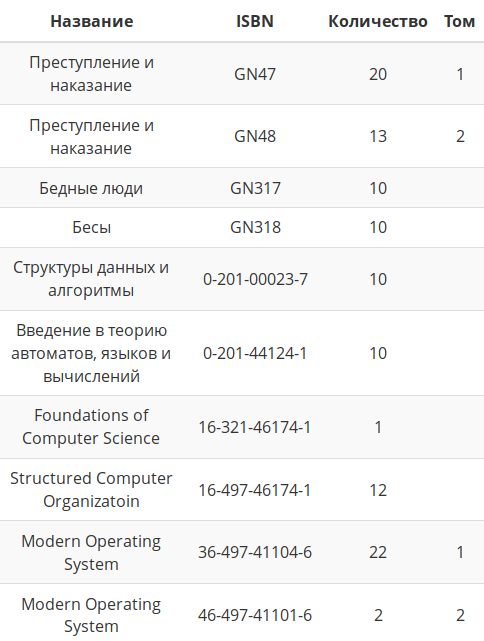
\includegraphics[scale=0.60]{images/search-result2.png} \\ а) Большой экран
\end{minipage}
\hfill
\begin{minipage}[h]{0.49\linewidth}
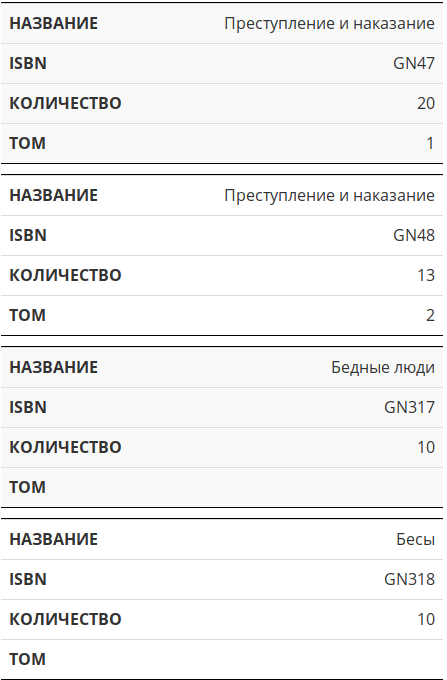
\includegraphics[scale=0.60]{images/search-result-adaptive.png} \\ б) Маленький экран
\end{minipage}
\caption{Адаптивная таблица результатов поиска.}
\label{ris:adaptive-table}
\end{figure}

Теперь немного изменим внешний вид всего приложения. Перенесем боковую
панель на правую сторону и перекрасим заголовки в зеленые цвета.

Откроем файл \texttt{theme.sass} где описана цветовая схема страниц.
В переменной \texttt{navbar-inverse-bg} находится основной цвет залоговков.
В базовой версии проекта уже настроена цветовая зависимость компонентов
страницы от этого цвета. Нам всего лишь необходимо его поменять на желаемый.

Перейдем к описанию стилей для боковой панели. Оно находится в
файле \texttt{sidebar.sass}.

Изначально боковое меню занимает позицию слева от
основного содержимого страницы. Необходимо изменить значения
\texttt{left} на \texttt{right}. Но это еще не все.
При скрытии или при разворачивании меню контейнер для основного содержимого
получал или убирал внутренние поля с левой стороны
в размере ширины бокового меню.

Заменим это поведение на противоположное. Внутренние поля теперь
будут изменяться с правой стороны контейнера.

Само меню переключалось по нажатию небольшой кнопки расположенной
в области основного контента, которая добавляла или удаляла
класс \texttt{toggled} у всей страницы. Тоже перенесем ее
в правую часть родительского контейнера.

Осталось только внести соответствующие изменения в медиа-запрос,
в котором боковое меню при получении страницы класса-переключателя
должно вести себя с точностью до наоборот.

\begin{figure}[ht!]
\begin{center}
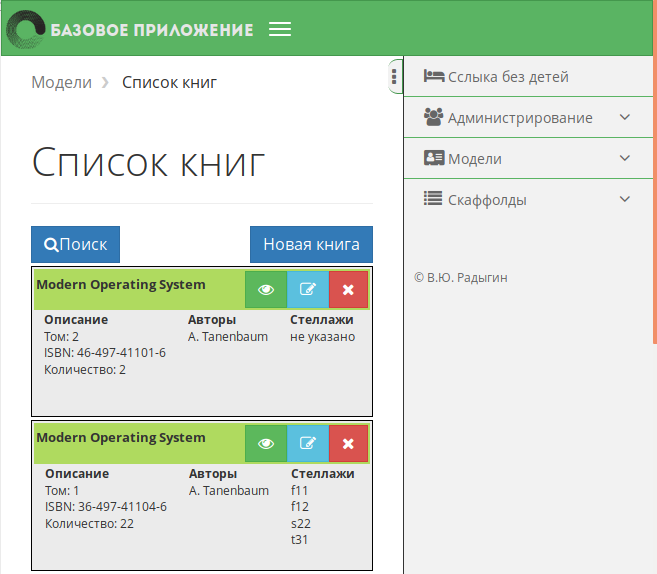
\includegraphics[scale=0.75]{images/sidebar.png}
\end{center}
\vspace*{-8mm}
\caption{Боковое меню справа} \label{fig:sidebar}
\end{figure}

На данном этапе в проекте реализован работоспособный поиск
\verb|Книг|, включая не только ее собственные атрибуты, но и те, которые
доступны ей по транзитивным связям. Результат поиска
оформлен в виде адаптивной таблицы. Выполнено задание по внешнему оформлению
проекта.
